\section{Referencia de la Clase Albaranes\-Proveedor}
\label{classAlbaranesProveedor}\index{AlbaranesProveedor@{AlbaranesProveedor}}
Clase que almacena la informaci\'{o} de los albaranes de proveedor.  


{\tt \#include $<$albaranesproveedor.h$>$}

Diagrama de colaboraci\'{o}n para Albaranes\-Proveedor:\begin{figure}[H]
\begin{center}
\leavevmode
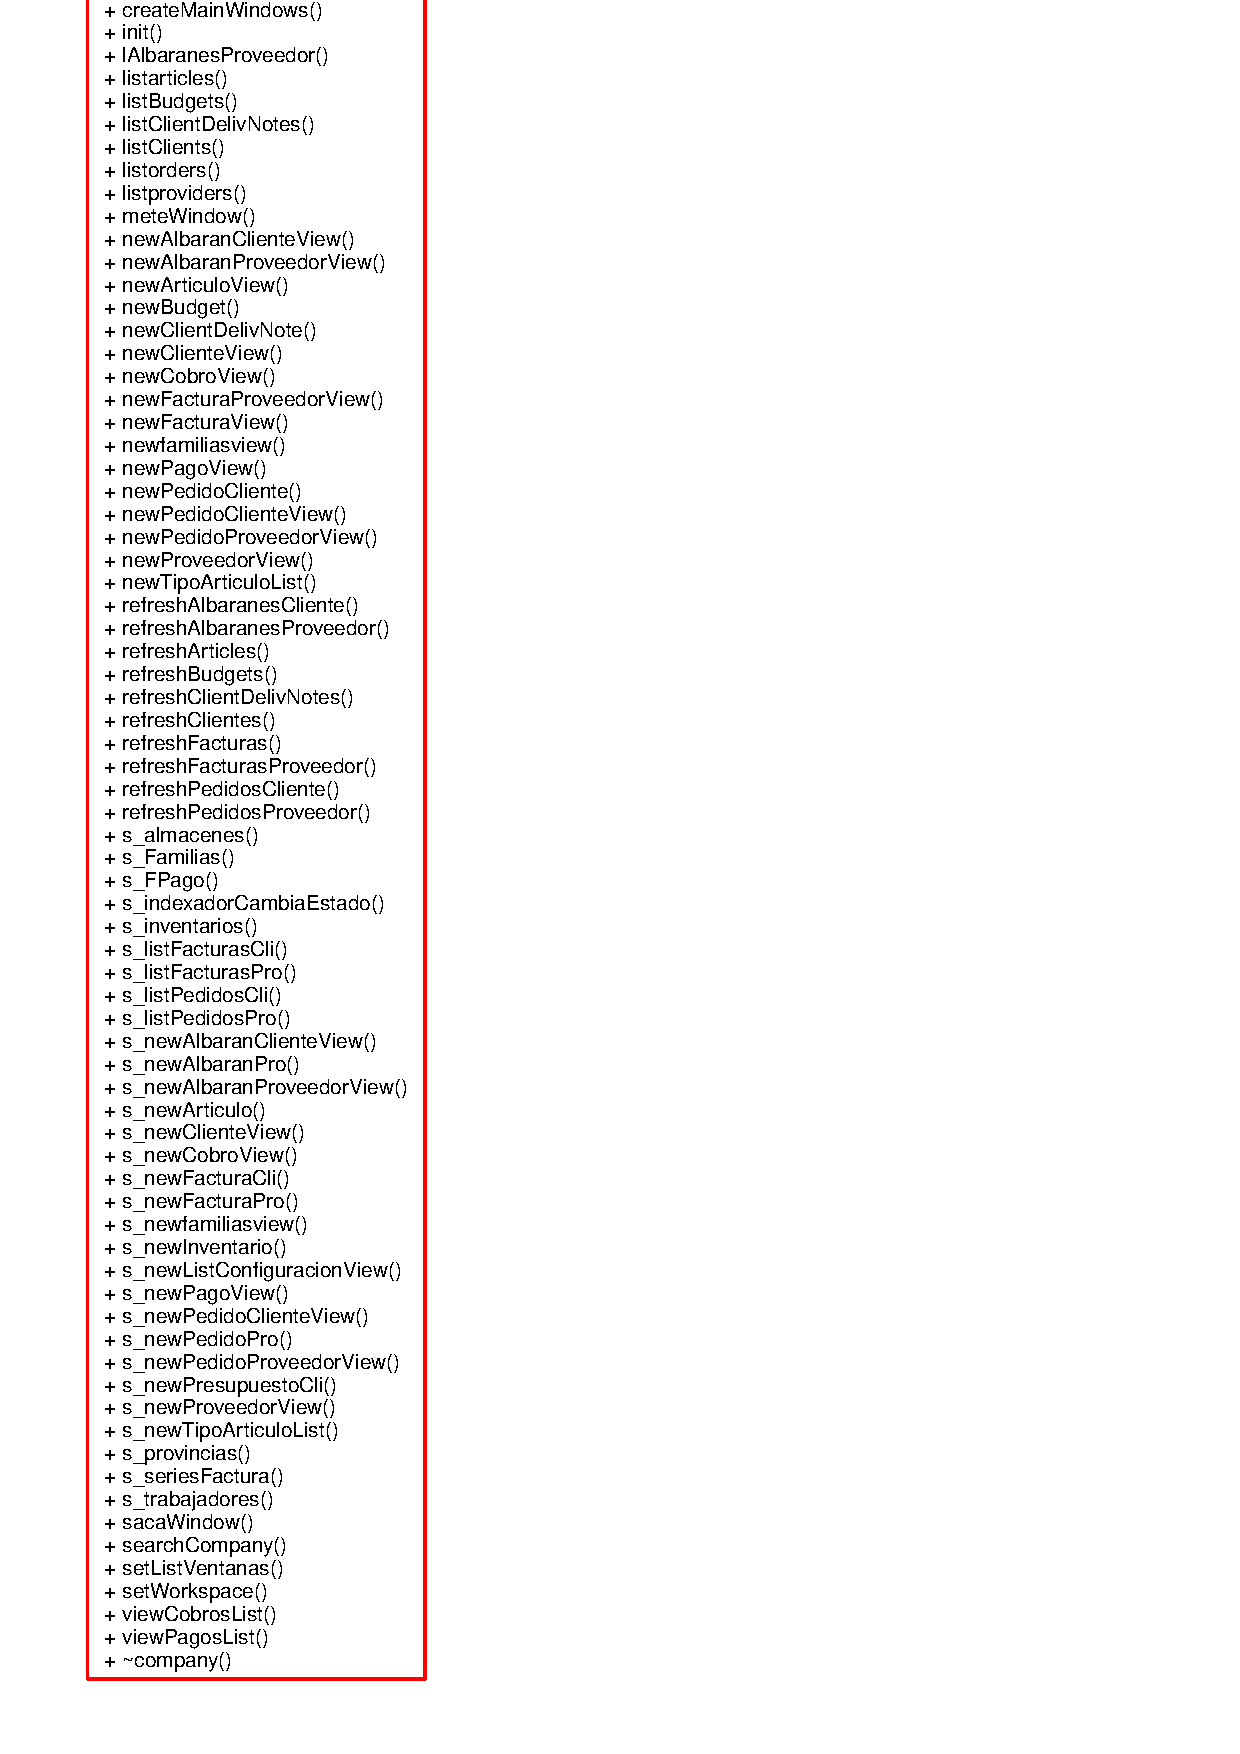
\includegraphics[width=131pt]{classAlbaranesProveedor__coll__graph}
\end{center}
\end{figure}
\subsection*{Slots p\'{u}blicos}
\begin{CompactItemize}
\item 
virtual void {\bf on\_\-m\_\-filtro\_\-text\-Changed} (const QString \&text)\label{classAlbaranesProveedor_i0}

\item 
virtual void {\bf on\_\-mui\_\-actualizar\_\-clicked} ()\label{classAlbaranesProveedor_i1}

\item 
virtual void {\bf on\_\-mui\_\-borrar\_\-clicked} ()\label{classAlbaranesProveedor_i2}

\item 
virtual void {\bf on\_\-mui\_\-configurar\_\-toggled} (bool checked)\label{classAlbaranesProveedor_i3}

\item 
virtual void {\bf on\_\-mui\_\-crear\_\-clicked} ()\label{classAlbaranesProveedor_i4}

\item 
virtual void {\bf on\_\-mui\_\-editar\_\-clicked} ()\label{classAlbaranesProveedor_i5}

\item 
virtual void {\bf on\_\-mui\_\-imprimir\_\-clicked} ()\label{classAlbaranesProveedor_i6}

\item 
void {\bf on\_\-mui\_\-list\_\-item\-Double\-Clicked} (QTable\-Widget\-Item $\ast$)\label{classAlbaranesProveedor_i7}

\end{CompactItemize}
\subsection*{Se\~{n}ales}
\begin{CompactItemize}
\item 
void {\bf selected} (QString)\label{classAlbaranesProveedor_l0}

\end{CompactItemize}
\subsection*{M\'{e}todos p\'{u}blicos}
\begin{CompactItemize}
\item 
{\bf Albaranes\-Proveedor} ({\bf company} $\ast$comp=NULL, QWidget $\ast$parent=0, Qt::WFlags flag=0)\label{classAlbaranesProveedor_a0}

\item 
{\bf Albaranes\-Proveedor} (QWidget $\ast$parent=0, Qt::WFlags flag=0)\label{classAlbaranesProveedor_a1}

\item 
void {\bf editar} (int)\label{classAlbaranesProveedor_a2}

\item 
QString {\bf genera\-Filtro} ()
\item 
void {\bf hide\-Botonera} ()\label{classAlbaranesProveedor_a4}

\item 
void {\bf hide\-Busqueda} ()\label{classAlbaranesProveedor_a5}

\item 
QString {\bf idalbaranp} ()\label{classAlbaranesProveedor_a6}

\item 
void {\bf imprimir} ()\label{classAlbaranesProveedor_a7}

\item 
void {\bf mete\-Window} (QString nom, QObject $\ast$obj)\label{classAlbaranesProveedor_a8}

\item 
void {\bf modoedicion} ()\label{classAlbaranesProveedor_a9}

\item 
void {\bf modoseleccion} ()\label{classAlbaranesProveedor_a10}

\item 
void {\bf presenta} ()
\item 
void {\bf setcompany} ({\bf company} $\ast$comp)\label{classAlbaranesProveedor_a12}

\item 
void {\bf setidarticulo} (QString val)\label{classAlbaranesProveedor_a13}

\item 
void {\bf setidproveedor} (QString val)\label{classAlbaranesProveedor_a14}

\item 
void {\bf show\-Botonera} ()\label{classAlbaranesProveedor_a15}

\item 
void {\bf show\-Busqueda} ()\label{classAlbaranesProveedor_a16}

\end{CompactItemize}


\subsection{Descripci\'{o}n detallada}
Clase que almacena la informaci\'{o} de los albaranes de proveedor. 



\subsection{Documentaci\'{o}n de las funciones miembro}
\index{AlbaranesProveedor@{Albaranes\-Proveedor}!generaFiltro@{generaFiltro}}
\index{generaFiltro@{generaFiltro}!AlbaranesProveedor@{Albaranes\-Proveedor}}
\subsubsection{\setlength{\rightskip}{0pt plus 5cm}QString Albaranes\-Proveedor::genera\-Filtro ()}\label{classAlbaranesProveedor_a3}


Tratamiento de los filtros. \index{AlbaranesProveedor@{Albaranes\-Proveedor}!presenta@{presenta}}
\index{presenta@{presenta}!AlbaranesProveedor@{Albaranes\-Proveedor}}
\subsubsection{\setlength{\rightskip}{0pt plus 5cm}void Albaranes\-Proveedor::presenta ()}\label{classAlbaranesProveedor_a11}


Hacemos el calculo del total. 

La documentaci\'{o}n para esta clase fu\'{e} generada a partir de los siguientes archivos:\begin{CompactItemize}
\item 
albaranesproveedor.h\item 
albaranesproveedor.cpp\end{CompactItemize}
